
\title{Electricity system}
% Use \titlerunning{Short Title} for an abbreviated version of your contribution title if the original one is too long
\author{Juan Van Roy, Bart Verbruggen and Johan Driesen}
\authorrunning{J. Van Roy, B. Verbruggen, J. Driesen}
\institute{Bart Verbruggen \at K.U.Leuven, Kasteelpark Arenberg 10 bus 2445, BE-3001 Leuven (Heverlee) \email{bart.verbruggen@esat.kuleuven.be}
\and Juan Van Roy \at K.U.Leuven, Kasteelpark Arenberg 10 bus 2445, BE-3001 Leuven (Heverlee) \email{juan.vanroy@esat.kuleuven.be}}

\maketitle

\abstract{A numeric electric system model is developed in Modelica for integrated energy simulation.}

\vspace{\baselineskip}

In this section, we describe in detail the electrical models that are implemented in Modelica as part of the IDEAS platform. These are models on the production, electrical distribution and storage side. First the photovoltaic (PV) system is treated which produces electricity locally from solar energy. In a second part, the distribution of electricity on distribution level is described.

Work in progress are the in-home electricity grid and the electrical storage in batteries.

\section{Photovoltaic system}
First, a photovoltaic (PV) system is implemented based on the five parameter model to simulate the energy production from a photovoltaic system. The five parameter model, which is temperature dependent, is based on the single diode equivalent circuit of a PV panel~\cite{desoto,sera}. The five parameters are:
\begin{itemize}
\item the light current, $I_{ph}$;
\item the diode reverse saturation current, $I_{o}$;
\item a shunt resistance, $R_{sh}$;
\item a series resistance, $R_{s}$;
\item the thermal voltage, $V_{t}$.
\end{itemize} 
These parameters are indicated in the equivalent circuit presented in Figure~\ref{fig:5param_equiv}.

\begin{figure}[ht]
\centerline{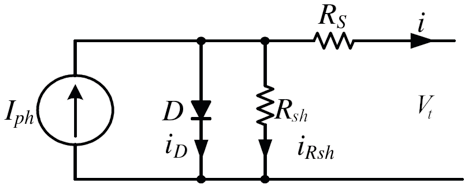
\includegraphics[width=0.5\textwidth]{Electric/MyGraphics/5param_eq.png}}
\label{fig:5param_equiv}
\caption{Five parameter model of a PV panel~\cite{desoto}} 
\end{figure}

\subsection{Power output of PV panel}
The electrical output from a PV system depends on the solar radiation, the ambient temperature of the cells, the solar incidence angle and the load. The solar radiation, incidence angle and temperature is obtained from chapter \ref{chap:climate}. The parameters needed for the model can generally be obtained from data gathered from the manufacturer's specifications of the solar panels. The required specifications to calculate the five parameters are the current $I_{mpp}$ and voltage $V_{mpp}$ at maximum power point (mpp) under standard testing conditions (STC)\footnote{Standard testing conditions are $(i)$ an irradiance of 1000 W/m$^2$ and $(ii)$ a cell temperature of 25$^\circ$C and $(iii)$ reference air mass of 1.5}, the short circuit current $I_{sc}$ and open circuit voltage $V_{oc}$ under the same standard testing conditions, the temperature coefficients $k_{i}$ and $k_{v}$ of respectively the short circuit current and open circuit voltage and the nominal cell temperature under STC $T_{c,ref}$.

The general current-voltage ($i-v$) equation for the single diode equivalent circuit is given in Eq.~(\ref{eq1}). 

\begin{equation}
i = I_{ph} - I_{0} \biggl(e^{\frac{v + i R_{s}}{n_{s} V_{t}}} - 1 \biggr) - \frac{v + i R_{s}}{R_{sh}}
\label{eq1}
\end{equation}

In this equation $V_{t}$ is the junction thermal voltage and $n_{s}$ the number of cells in the panel connected in series:
\begin{equation}
V_t = \frac{A k T_{stc}}{q}
\label{eqVt}
\end{equation}

with $A$ the ideality factor, $k$ the Boltzmann's constant ($1.380663 \cdot 10^{-23}$ J/K), $q$ the charge of an electron ($1.600218 \cdot 10^{-19}$ C) and $T_{stc}$ the cell temperature under STC.

The voltage $V_{mpp}$ and current $I_{mpp}$ at maximum power point should satisfy this equation and according to Eq.~(\ref{eq2}), the derivative of the power with respect to the voltage should be zero at this point. Eq.~(\ref{eq3}) states that the derivative of the current with respect to the voltage at short circuit current should be the negative of the shunt conductance ($1/R_{sh}$). These equations lead to the calculation of the parameters $R_{s}$, $R_{sh}$ and $V_{t}$.

\begin{equation}
\frac{dP}{dV} \Bigr\vert_{\substack{V=V_{mpp},~I=I_{mpp}}} = 0
\label{eq2}
\end{equation}
\begin{equation}
\frac{dI}{dV} \Bigr\vert_{I = I_{sc}} = - R_{sh}^{-1}
\label{eq3}
\end{equation}

The maximum power point $P_{mpp}$ can be found with Eq.~(\ref{pmpp}):
\begin{equation}
\frac{dP}{dV} \Bigr\vert_{\substack{I=I_{mpp}}} = I_{mpp} + V_{mpp} \frac{-\frac{(I_{sc} R_{sh} - V_{oc} + I_{sc} R_{s}) e^{\frac{V_{mpp} + I_{mpp} R_{s} - V_{oc}}{n_{s} V_{t}}}}{n_{s} V_{t} R_{sh}} - \frac{1}{R_{sh}}}{1 + \frac{(I_{sc} R_{sh} - V_{oc} + I_{sc} R_{s}) e^{\frac{V_{mpp} + I_{mpp} R_{s} - V_{oc}}{n_{s} V_{t}}}}{n_{s} V_{t} R_{sh}} + \frac{R_{s}}{R_{sh}}}
\label{pmpp}
\end{equation}

The reverse saturation current $I_{o}$ and light current $I_{ph}$ at STC can be found based on Eq.~(\ref{eq1}) for the short circuit (Eq.~(\ref{eq4})) and open circuit condition (Eq.~(\ref{eq5})).
\begin{equation}
I_{sc} = I_{ph} - I_{0} e^{\frac{I_{sc} R_{s}}{n_{s} V_{t}}} - \frac{I_{sc} R_{s}}{R_{sh}}
\label{eq4}
\end{equation}
\begin{equation}
I_{oc} = 0 = I_{ph} - I_{0} e^{\frac{V_{oc}}{n_{s} V_{t}}} - \frac{V_{oc}}{R_{sh}}
\label{eq5}
\end{equation}

The five parameter model is implemented in a Modelica model to calculate the power output of the photovoltaic panels under operational conditions. The current and voltage at maximum power point can be found by solving Eqns.~(\ref{eq1}) and~(\ref{eq2}) for the non-reference conditions. The parameters for these conditions are calculated in the next paragraphs.

The PV parameters are adjusted to take into account the position of the sun, the direct and indirect radiation and the ambient temperature. The cell temperature has been adjusted to be the ambient temperature plus the losses of the panel.

The tilt angle and orientation of the PV panels are parameters of the PV model. Together with the sun's position, the incidence angle of the direct beam radiation can be calculated which allows to obtain the amount of radiation that gets reflected by and passes through the PV panel cover. This is done using incidence angle modifiers that are derived from De Soto et al.~\cite{desoto}. The incidence angle modifier $K_{\tau \alpha}(\theta)$ can be found from the transmittance $\tau$ of the cover system with Eq.~(\ref{eq8}), which is approximated in Eq.~(\ref{eq7}). The angle of refraction, $\theta _{r}$, is determined in Eq.~(\ref{eq6}) by Snell's law, with $\theta$ the incidence angle and $n$ the effective index of refraction of the cell cover. In Eq.~(\ref{eq7}), $K$ is the glazing extinction coefficient and $L$ is the glazing thickness. In the model $K$ and $L$ can be adjusted. By default, $K$ is assumed to be $4~m^{-1}$ and $L$ is assumed to be $2~mm$.
\begin{equation}
\theta _{r} = arcsin(n \cdot sin \theta)
\label{eq6}
\end{equation}
\begin{eqnarray*}
\tau (\theta) & = & e^{-\frac{K~L}{cos \theta _{r}}} \biggl[1 - \frac{1}{2} \biggl(\frac{sin^{2}(\theta _{r} - \theta)}{sin^{2}(\theta _{r} + \theta)} + \frac{tan^{2}(\theta _{r} - \theta)}{tan^{2}(\theta _{r} + \theta)} \biggr) \biggr]
\label{eq7}
\end{eqnarray}
\begin{equation}
K_{\tau \alpha}(\theta) = \frac{\tau (\theta)}{\tau (0)}
\label{eq8}
\end{equation}

The incidence angle modifiers and the direct and diffuse radiation, which are inputs to the model, allow together with the reflected radiation to calculate the absorbed solar radiation $S$ in Eq.~(\ref{eq9}). In this equation $G_{b}$ is the direct, $G_{d}$ the diffuse and $G$ the total radiation. The slope of the PV panel is characterized by $\beta$.
\begin{eqnarray*}
\frac{S}{S_{ref}} & = & \frac{G_{b}}{G_{ref}} K_{\tau \alpha , b} + \frac{G_{d}}{G_{ref}} K_{\tau \alpha , d} \frac{1 + cos \beta}{2} + \frac{G}{G_{ref}} \rho K_{\tau \alpha , g} \frac{1 - cos \beta}{2}
\label{eq9}
\end{eqnarray}

with
\begin{equation}
S_{ref} = G_{ref} e^{-K \cdot L}
\label{eqSref}
\end{equation}

and $G_{ref}$ is the irradiance at STC (1000 W/m$^2$).

The light current $I_{ph}$, reverse saturation current $I_{0}$ and thermal voltage $V_{t}$ at non-reference conditions can be calculated when the temperature, open circuit voltage and short circuit current are known~\cite{sera}. The open circuit voltage $V_{oc}$ can be calculated using Eqns.~(\ref{eq10}) and~(\ref{eq11}). The short circuit current $I_{sc}$ can be found using Eq.~(\ref{eq12}).
\begin{equation}
e^{\frac{V_{oc}(S)}{n_{s} V_{t}}} = \frac{I_{ph}(S) R_{sh} - V_{oc}(S)}{I_{0} {R_{sh}}}
\label{eq10}
\end{equation}
\begin{equation}
V_{oc}(T) = V_{oc} + k_{v} (T - T_{stc})
\label{eq11}
\end{equation}
\begin{equation}
I_{sc}(S,T) = I_{sc} \biggl(\frac{S}{S_{ref}} \biggr) \biggl(1 + \frac{k_{i}}{100} (T - T_{ref}) \biggr)
\label{eq12}
\end{equation}

The reverse saturation current $I_{0}$ can be calculated with Eq.~(\ref{eq13}). The light current $I_{ph}$ is found using Eq.~(\ref{eq14}).
\begin{equation}
I_{0} = \biggl(I_{sc} - \frac{V_{oc} - I_{sc} R_{s}}{R_{sh}} \biggr) e^{-\frac{V_{oc}}{n_{s} V_{t}}}    
\label{eq13}
\end{equation}
\begin{equation}
I_{ph} = I_{0} e^{\frac{V_{oc}}{n_{s} V_{t}}} + \frac{V_{oc}}{R_{sh}}
\label{eq14}
\end{equation}

\subsection{Power output of PV system}
A PV system consists of multiple PV panels connected in series. Assuming that all PV panels are in the same condition, the output DC voltage can be multiplied by the number of PV panels in a PV system.

The number of PV panels is a parameter of the general PV system model. The peak power $P_{peak}$ is defined with $V_{mpp}$, $I_{mpp}$ and the number of panels $n_p$:
\begin{equation}
P_{peak} = n_p V_{mpp} I_{mpp}
\label{Ppeak}
\end{equation}

\subsection{Orientation PV system}
The PV system has two orientation parameters, namely $(i)$ the azimuth and $(ii)$ the inclination angle. An azimuth angle of 0$^\circ$ is defined as towards the South, -90$^\circ$ for the East and 90$^\circ$ for the West. Applied to Belgium, the PV system has the highest annual electricity production when the system is oriented directly to the South with an inclination of 34$^\circ$.

\subsection{Inverter}
A PV system is connected to the electrical grid through an inverter, which converts the generated DC power to AC power with an efficiency $\eta_{dc/ac}$.

Due to the lack of simultaneity of production and consumption, a bidirectional energy flow may occur between a building and the electrical grid (e.g. low voltage grid for residential buildings), which may lead to voltage instabilities on the grid (e.g. increasing voltages due to the injection of electricity, unbalance, etc.). To avoid excessive feeder voltages at the moments of re-injecting PV power in the grid, the inverter is curtailed when a predefined voltage limit is reached. Curtailing of a PV system means production losses.

According to the AREI\footnote{Algemeen Reglement voor Elektrische Installaties, Belgi\"e.}, Art.235, this limit is 6 \% above the nominal voltage (230 V in Belgium). A certain minimal off-time is given before reconnecting the inverter to the grid. Synergrid states that PV systems are curtailed when the average grid voltage at the connection point of the building (during 10 minutes) reaches a predefined voltage of 230 + 10 \% V)~\cite{synergrid}. An instant switch-off is required when the voltage reaches 230 + 15 \% V. In principle, the strictest rule has to be followed. In this case, there is an agreement that the values of Synergrid can be followed until the AREI is adapted.

\section{Electrical distribution grid}
An electrical distribution grid for low voltage (e.g. 230/400 V wye, or star connection) is modeled. Both a 1-phase en 3-phase grid can be simulated. The 1-phase grid can serve for fully balanced simulations.

In the electrical grid system two types of grids exist, namely $(i)$ distribution and $(ii)$ transmission grids~\cite{ehaesen,willis}. However, in Belgium, distribution grids differ fundamentally from transmission grids:

\begin{itemize}
\item They are mostly radially: This means there is only one feeding transformer\footnote{Traditionally, there is only a unidirectional power flow.}. Due to the lack of a redundant supply, the reduced reliability is a major disadvantage. In case of a fault, all loads behind the fault will be switched off.
\item The lower the voltage level, the higher the R/X ratio\footnote{R = resistance, X = reactance}. Thus, low voltage residential distribution grids are highly resistive.
\end{itemize}

First, the grid topology is described. As will be shown, any radial grid can be easily represented by two matrices, namely the incidence and impedance matrix. Second, the background for the power flow analysis will be described to determine the nodal currents, line currents and nodal voltages. Radial grids are generally more easy to analyze and because of the low cost, it is prefered for distribution grids~\cite{ehaesen}.

\subsection{Grid topology}


\subsection{Power flow analysis}

\section{Electrical in-home grid}
In progress.

\section{Electrical storage}
In progress.